\documentclass{cta-author}

\usepackage{amsmath,amssymb,amsfonts}
\usepackage{algorithm}
\usepackage{algpseudocode}
\usepackage{graphicx}
\usepackage{textcomp}
\usepackage{multirow}
\usepackage[export]{adjustbox}

\newtheorem{theorem}{Theorem}{}
\newtheorem{corollary}{Corollary}{}
\newtheorem{remark}{Remark}{}

\begin{document}

	% New definitions
  \algnewcommand\algorithmicswitch{\textbf{switch}}ep
  \algnewcommand\algorithmiccase{\textbf{case}}
  \algnewcommand\algorithmicassert{\texttt{assert}}
  \algnewcommand\Assert[1]{\State \algorithmicassert(#1)}%
  % New "environments"
  \algdef{SE}[SWITCH]{Switch}{EndSwitch}[1]{\algorithmicswitch\ #1\ \algorithmicdo}{\algorithmicend\ \algorithmicswitch}%
  \algdef{SE}[CASE]{Case}{EndCase}[1]{\algorithmiccase\ #1}{\algorithmicend\ \algorithmiccase}%
  \algtext*{EndSwitch}%
  \algtext*{EndCase}%

\supertitle{Submission Template for IET Research Journal Papers}

\title{I am still here}

\author{\au{First Author$^{1}$}, \au{Second Author$^{2\corr}$}, \au{Third Author$^{3}$}}

\address{\add{1}{First Department, First University, Address, City, Country Name}
\add{2}{Second Company Department, Company Address, City, Country Name}
\add{3}{Third Department, Third University, Address, Country Name}
\add{4}{Current affiliation: Fourth Department, Fourth University, Address, Country Name}
\email{corresponding.author@second.com}}

\begin{abstract}
This should be informative and suitable for direct
inclusion in abstracting services as a self-contained
article. It should not exceed 200 words. It should
summarise the general scope and also state the main results
obtained, methods used, the value of the work and the
conclusions drawn. No figure numbers, table numbers,
references or displayed mathematical expressions should be
included. The abstract should be included in both the
Manuscript Central submission step (Step 1) and the
submitted paper.
\end{abstract}

\maketitle

\section{Introduction}\label{sec:intro}
As sensor networks, distributed system, and Internet of Things (IoTs) are the physical endpoints of a healthcare application, a number of traditional healthcare strategies has been becoming online healthcare systems service.
In fact, global healthcare organizations make a change of their data into Electronic Patient Health Records (EPHR).
%In fact, there are more and more global healthcare organizations that make change of their data into Electronic Patient Health Records (EPHR). 
In Barack Obama's speech at the American Medical Association 2009, he mentioned that all the medical information should be stored securely in a private medical record \cite{zhang2014role}. 
Accordingly, a patient's information can be tracked from multiple doctors, even that patient has changed his/her hospital and specialists.
However, the interaction among patients, doctors, insurance companies, and pharmaceutical ones supported by healthcare systems are challenging problems. 
In fact, the sensitive nature of the information managed by healthcare systems requires the balance between two contrasting needs: demands for the availability of data to ensure the highest quality to patients and for the security of sensitive data (chronic diseases, mental health issues, psychiatric care, sexual behavior, fertility issues, abortion status, or HIV status...). 
Therefore, the core concern of the management systems is to prevent sensitive data from unauthorized access. 
According to that, access control (AC), a primary type of mechanism, is being applied by healthcare systems to protect the data. 
However, the traditional access control models are rigid, so it is challenging to apply them to the medical environment. 
%On the other hand, it was assumed that these security system policies have to be. 
Nevertheless, one of the most specific unbroken requests of medical data is "nothing interferes with the delivery of care" \cite{grandison2007impact}, with restricted access control would likely be ignored in emergency situations or other similar exceptions. 
For instance, in urgent ones, a nurse can request (and must be authorized) access to the data, which "normal" conditions she cannot view. 
This phenomenon is known as "break the glass" (BTG).

%What is considerably needed is the interaction among patients, doctors, insurance companies and pharmaceutical ones supported by healthcare systems. 
%The sensitive nature of the information managed by these systems requires the balance between two contrasting needs: demands for data to ensure the highest quality to the patients "availability" and for sensitive data security (chronic diseases, mental health issues, psychiatric care, sexual behavior, fertility issues, abortion status, and HIV status).
%Therefore, the core concern of the management systems is to preventing sensitive data from unauthorized access. 
%Access control (AC), a primary type of mechanism is being applied by these healthcare systems into protecting the data. 
%However, the traditional AC models is rigid, so it is difficult to apply them to the medical environment.
%On the other hand, one of the most specific unbroken requests of medical data is "nothing interferes with the delivery of care" \cite{grandison2007impact}, with restricted access control would likely be ignored in emergency situations. 
%For example, in urgent ones, a nurse can request (and must be authorized) access to the data, which "normal" conditions she cannot view. 
%This phenomenon is known as "break the glass" (BTG).

%Beforehand, there were numerous studies which could be considered as an application to BTG in terms of emergency/exception situation as a compulsory requirement in healthcare systems \cite{joint2004cocir}. 
%The model "Break The Glass" is kept separated from the basic access control model which was suggested by Petritch et al. \cite{petritsch2014generic}. 
%It allows users to override the consequence of access control; thus, a user can access resources that were not authorized earlier. 
%According to Ferreira et al. \cite{ferreira2009securely}, it supplies a third option, BTG, in addition to grand and deny; 
%the BTG option grants permission to authorized users to break the glass rather than denying access.
%Additionally, Ferreira has introduced the BTG integration method into the RBAC model with Obligations  \cite{ferreira2006break}. 
%In addition, some obvious flaws were found in this model. In the BTG state, users can not only override access control results (the user is granted greater authority), but they also ignore the system constraints, resulting in significant damage to the system. 
%To prevent such misuses the access control system should maintain its strictness under any circumstances. 
%In other words, it should be that the access control will not harm the security level of EPHR even in urgent situations where minimum levels of a security requirement are always present no matter how much serious the situation is \cite{gope2016novel}. 

Numerous studies have been done for applied BTG, in terms of emergency situation, as a compulsory requirement in healthcare systems \cite{joint2004cocir}.
The model "Break The Glass" is kept separated from the basic access control model suggested by Petritch et al. \cite{petritsch2014generic}. 
The model allows users to override the consequence of access control; thus, a user can access non-authorized resources. 
According to Ferreira et al. \cite{ferreira2009securely} BTG, in addition to two decision options Grant or Deny, grants permission to authorized users to break the glass instead of denying access.
Additionally, Ferreira introduced a different BTG policies application in comparison with traditional ones, offering users unlimited access and responsibility under unsecured situations \cite{ferreira2006break}.
In addition, some obvious flaws were found in this model. 
In the BTG state, users can not only override access control results (the user is granted greater authority), but they also ignore the system constraints, resulting in significant damage to the system. 

Variety approaches to prevent BTG's weaknesses, in the event of emergency or exception, have been suggested such as: minimizing possible cases lead to BTG, 
%RBAC extended model for the healthcare system, 
protecting medical data by cryptography functions, and defining the special policy for the emergency situation (BTG policy, policy spaces). 
%Maw et al. \cite{maw2014survey} stated that although a considerable access control models have been proposed for the healthcare system, some of them has not been implemented.
Nonetheless, the above mentioned methods have not completely overcome BTG in emergency situations. 
In this paper, the main aim is an introduction to an approach to prevent current shortages by providing privacy policy in both Normal and Emergency Situations, followed two criteria: the availability of data and the secured nature of the sensitive data.
%To do this, there are both two groups of users in parallel existence; first, an administrator usually takes a role in system management so as to give \texttt{system policies}; second, the patients who make a major contribution to create \texttt{sensitive data policy}.
In order to achieve this aim, two groups of users are considered in parallel existence: administrators participating in the system management to provide \texttt{system policies} and patients contributing to create \texttt{sensitive data policy}.
%One special feature of this approach is that we give permission the administrators and patients to change (insert, delete and edit) their policy. 
%The prime goal is to increase the flexibility of the system and adapt quickly to the complex healthcare institution where people change their roles and departments frequently \cite{ferreira2006break}. 
%About addressing the solution for this problem, we applied a flexible access control model to support special cases, which were by far extended from previous our work in "Dynamic Policy Environment"  \cite {son2016rew,son2017rew}. 
%Details of how the system works and the relationship between the two types of policy will be discussed in the next sections. 
By this approach, administrators and patients are allowed to modify (insert, delete and edit) their policies in the real-time.
% without any constraints on the part of the system.
The primary goal is to increase the flexibility of the system and to adapt quickly to the complex healthcare institution where people change their roles and departments frequently \cite{ferreira2006break}.
Obviously, healthcare systems are more and more being extended; therefore, dynamically updated policy support is essential.
Nevertheless, as the best of our knowledge, it has not been any research direction that drives policy change into adapting the healthcare system change.
A flexible access control model is applied to support special cases, which is followed by the approach in previous researches \cite{son2016rew,son2017rew}. 
%Details of the system and the relationship between the two types of policy will be discussed in the next sections. 
In this paper, we propose a policy change solution in order to meet the demands of privacy and flexibility in the healthcare system.
The contributions of this work includes the following:
\begin{itemize}
  \item Minimize emergency situations leading to BTG.
  \item Introduce appropriate rules and policies for medical data.
  \item Provide access control mechanisms in an appropriate dynamic policy environment for healthcare systems. 
  \item Provide a timely response mechanism when a policy update occurs.
  \item Implement our proposed theoretical model.
\end{itemize}

The rest of the paper is organized as follows:
In the next section, we provide relevant background material.
In section 3, we demonstrate our proposed model and implementation.
In the following sections, we evaluate our implementation based on security analysis, compared with the other models and measuring performance.
The next section is devoted to the prior work and then will conclude the paper with a summary of our results and discuss opportunities for further research in conclusion.

\section{Background}\label{sec:back}

%This part of the paper will introduce background knowledge, based on this knowledge that readers easily understand the later parts of the article.
\subsection{Encoding Policy}\label{Back:encoding-policy}
%delete Def 2 and 3, change new position for Def 1
This section is focused on an overview of the policies included in the system.
Policies can be formatted in JSON \cite{thi2017using} or XML\cite{rissanen2013extensible} depending on the defined system.
%However, with the initial policies structure, it is very difficult for the system to detect updates when a change occurs.
With the initial policies structure, an update is difficult to be detected by system.
%Thus, we first present a transformation of policies that flattens the hierarchical structure of a policy while preserving the semantics of the original policy. 
A transformation of policies is presented  to flattens the hierarchical structure of a policy while preserving the semantics of the original policy. 

%Next we present a sample policy, which is used as a running example throughout the paper.
The policy is ordered into 3 levels: \textit{PolicySet, Policy} and \textit{Rule}. 
Every elements can contain a \textit{Target}. The \textit{PolicySet} can contain the other \textit{PolicySet} or the set of \textit{Policys}.
The \textit{Policy} can contain the other \textit{Policy} or the set of \textit{Rules}.
On the other hand, the \textit{PolicySet} and \textit{Policy} has their \textit{Obligations} to fulfill whenever \textit{Response} is reached to either \textit{Permit} or \textit{Deny} decision. 
The following is presented the definitions and syntax of all elements.

Obligations $Os$ contain one or more obligation(s) $O$. 
An obligation is an action that takes place after a decision has been reached to either Permit or Deny.
It is mapped to ACDP-HC within the context of policy and policy set according to the following syntax:
\begin{equation}
	\textit{$Os::$}= \textit{$O\_set$}
\end{equation}
\begin{equation}
	\textit{$O::$}= \textit{$\langle OID, FF, {AID, DT, V} \rangle$}
\end{equation}
Where $Obligation\_set$ is the set of obligation ($O$). 
$OID$ is the ID identifying of obligation, $FF$ is the $fulfill$ (\texttt{On/Off}) attribute is a boolean function that is used as a key of determine when the obligation must be enforced and must be either permit or deny.  
$AID$ is the attribute ID of the obligation to be carried out. $DT$ is the data type and $V$ is the data value. 
If the policy or policy set being evaluated matches the $FF$ (\texttt{On}) attribute of its obligations, then the obligations are passed to be enforced otherwise obligations are ignored.

Target $T$ is an objective and is mapped to ACDP-HC within the context of rule, policy and policy set according to the following syntax:
\begin{equation}
	\textit{$T::$}= \textit{$\langle S, A, E, Rc \rangle $}
\end{equation}
Where $S$ is the set of subjects, $A$ is the set of actions, $E$ is the set of environments, and $Rc$ is the set of resources.

A rule $R$ is the most elementary element of a policy. 
A rule contains rule conditions, target and rule effect. 
It is mapped to ACDP-HC according to the following syntax:
\begin{equation}
	\textit{$R::$}= \textit{$\langle IDR, RC, T, Re \rangle$}
\end{equation}
Where $IDR$ is the identify of rule, $RC$ is the set of rule conditions, $T$ is the set of targets, and $Re$ is the rule effect.

A policy $P$ is a single access control policy. 
It is expressed through a set of rules. 
A policy contains a set of rules, rule combining algorithm, target and obligations.
It is mapped to ACDP-HC according to the following syntax:
\begin{equation}
	\textit{$P::$}= \textit{$\langle IDP, SR, RCA, T, Os \rangle$}
\end{equation}
Where $IDP$ is the identify of policy, $SR$ is the set of rules, $RCA$ is the rule combining algorithm, $T$ is the set of targets, and $Os$ is the set of obligations.

Policy set $PS$ is created by the set of policies $P$. $PS$ may contain other policy sets, policies or both. 
It is mapped to ACDP-HC according to the following syntax:
\begin{equation}
	\textit{$PS::$}= \textit{$\langle IDPS, SP, PCA, T, Os \rangle$}
\end{equation}		
Where $IDPS$ is the identify of policy set, $SP$ is the set of policies, $PCA$ is the policy combining algorithm, $T$ is the set of targets, and $Os$ is the set of obligations.

\subsection{Encoding Request}\label{Back:request}

A request \textit{Rq} is a requirement for access to some resources. It is mapped to ACDP-HC according to the following syntax:
\begin{equation}
	\textit{$Rq::$}= \textit{$\langle Sr, Ar, Rr, Er \rangle$}
\end{equation}
Where $Sr$ is the set of subjects, $Ar$ is the set of actions, $Rr$ is the set of resources and $Er$ is the set of environment information.

\subsection{Encoding Response}\label{Back:response}

A response \textit{Rs} is a decision to a request against a based policy 
It is mapped to ACDP-HC according to the following syntax:
\begin{equation}
	\textit{$Rs::$}= \textit{$\langle D, Os \rangle$}
\end{equation}
Where $D$ is the decision of the response and $Os$ is the set of obligations to be executed within the response. 

\subsection{Policy Translation}\label{Back:policy-translation}

\textbf{Policy Example :} In "\textbf{normal situation}", a doctor or nurse only have access to the patient information they receive on arrival only if they are present in the patient's treatment department need access. 
%The user group is an insurance company that is only allowed to access hospital's fee and ID number of patients, similarly to the pharmacy that allowed to access the ID number and prescription drug of patients. 
The other user group is insurance companies with limited access such as access to hospital's fee and ID number of patients; or the pharmacy with limited access such as the ID number and prescription drugs of patients.
In "\textbf{emergency situation}",when and only if the doctor or nurse who takes care of a patient is absent and the others want to access the medical data of this patient, it must be satisfied: either by the patient's agreement or possibly a family member/whom the patient fully trusts%or any information of the doctors or nurse practitioners (personal information, time, location, access reason) must be kept in the log system and be legally responsible for leaking the patient's information
\footnote{\textbf{Note: }The normal situation is used for all patient data areas and is managed by admin, while the emergency situation is managed by the patient, depending on the type of data that the patient needs different defenses that the policy defines. 
These policies are called if the data zone it is accessed in an emergency situation.
%Without this policy, the patient does not have to request personal data protection in an emergency situation so that data is easily provided to the doctors or nurses.}.
Without those policies, the patient does not own private data; hence, the data is easily accessed by responsible doctors or nurses.} 

In this example, the policy set includes policy elements and possibly combines these policies using \texttt{first-applicable (fa)}. One way to model the policy elements is to represent (the negation of) these constraints as  \texttt{Deny} rules. 
In addition, a default policy is introduced with effect \texttt{Permit} and combined using \texttt{deny-overrides (dov)}. 
According to  \texttt{dov}, the policy yields decision  \texttt{Permit} only if none of the \texttt{Deny} rules is applicable. 

%This policy set is represented in the notation as follows:

%\begin{equation}
%  \textit{$P(set)$}: \textit{$\langle p(set)[com\_al\_policy\_ID], p_1, p_2, \dots, p_n \rangle$}
%\end{equation}

%Where $p[com\_al\_policy\_ID]$ is the ID of combining algorithm policy and $p_1, p_2, \dots, r_n$ denoted from \texttt{policy 1} to \texttt{policy n}. As in the case of the \textit{policy set structure}, the \textit{policy structure} is defined as follows:

%\begin{equation}
%  \textit{$P$}: \textit{$\langle p[com\_al\_rule\_ID], r_1, r_2, \dots, r_m \rangle$}
%\end{equation}

The information of patients are included, for example, ID, name, gender, age, address, phone, drugs, health history, department, relation, hospital's fee, AvailableDoctorNurse, %determine the presence of doctors/nurses are present at the hospital, % and OwnEmergencyPolicy determine whether that patient owns sensitive data policy.
patientEmerAgree and relatPatientEmerAgree. %determine the patient's agreement and family member agreement in emergency situation.
AvailableDoctorNurse determines whether the presence of doctors/nurses are present at the hospital.
In the meantime, patientEmerAgree and relatPatientEmerAgree determine the patient's agreement and family member agreement in emergency situation.
The original policy set is represented in policies and rules as follows:

\textit{$\textbf{Policy\: set}::$}= \textit{$\langle  PS, \{P_1, P_2, P_3, P_4\}, first-applicabe, \{ \:, read, \:,\\ patients' record \}, \{ \} \rangle$}

\textit{$\textbf{Policy\:1}::$}= \textit{$\langle  P_1, \{R_1, R_2\}, deny-overrides, \{ \{ nurse,\: doctor\},\: ,\\ , \}, \{ \} \rangle$}

%$P_1[\textit{dov}] : subject : "nurse" \wedge "doctor"$

\textit{$\:\:\:\:\: \textbf{Rule\:1}::$}=\textit{$\langle R_1, availableNurseDoctor = \textbf{false}, \{,\: ,\: ,\: available\\NurseDoctor\}, Deny \rangle$}

\textit{$\:\:\:\:\: \textbf{Rule\:2}::$}=\textit{$\langle R_2, patientID \notin List\_Caring\_Patients, \{ ,\: ,\: ,\: patient\\ID\}, Deny \rangle$}

\textit{$\textbf{Policy\:2}::$}= \textit{$\langle  P_2, \{R_3\}, deny-overrides, \{insurance\:\:companies,\: ,\\, \}, \{ \} \rangle$}

%$P_2[\textit{dov}] : subject : "insurance \:\: companies" $

\textit{$\:\:\:\:\: \textbf{Rule\:3}::$}=\textit{$\langle R_3, patients' \:\: information \notin \{patientID,\:hospital's\\ \: fee\}, \{,\: ,\: ,\: \{patientID,\:hospitalFee\}\}, Deny \rangle$}

%$\:\:\:\:\: R_4[\textit{Deny}] : patients' \:\: information \notin \{ID,\:hospital's \: fee\}$

%$\:\:\:\:\: R_5[\textit{Permit}] : \textbf{true} $

\textit{$\textbf{Policy\:3}::$}= \textit{$\langle  P_3, \{R_4\}, deny-overrides, \{pharmacies,\: ,\:, \}, \{ \} \rangle$}

%$P_3[\textit{dov}] : subject :  "pharmacies"$

\textit{$\:\:\:\:\: \textbf{Rule\:4}::$}=\textit{$\langle R_4, patients' \:\: information \notin \{patientID,\:drug\},\\ \{,\: ,\: ,\: \{patientID,\:drug\} \}, Deny \rangle$}

%$\:\:\:\:\: R_6[\textit{Deny}] : patients' \:\: information \notin \{ID,\:drug\}$

%$\:\:\:\:\: R_7[\textit{Permit}] : \textbf{true} $

\textit{$\textbf{Policy\:4}::$}= \textit{$\langle  P_4, \{R_5, R_6\}, deny-overrides,  \{ \{ nurse,\: doctor\},\: ,\\ , \}, \{ \} \rangle$}

%$P_4[\textit{dov}] : subject : "nurse" = "doctor"$

\textit{$\:\:\:\:\: \textbf{Rule\:5}::$}=\textit{$\langle R_5, availableNurseDoctor = \textbf{true}, \{,\: ,\: ,\: available\\NurseDoctor\}, Deny \rangle$}

%$\:\:\: R_{8}[\textit{Deny}] : AvailableNurseDoctor = \textbf{true}$

\textit{$\:\:\:\:\: \textbf{Rule\:6}::$}=\textit{$\langle R_6, patientEmergencyAgreement = \textbf{false} \wedge related\\PatientEmergencyAgreement = \textbf{false}, \{,\: ,\: ,\: \{ patientEmergencyA\\greement, relatedPatientEmergencyAgreement\}\}, Deny \rangle$}

%$\:\:\: R_{9}[\textit{Deny}] : patientEmerAgree = \textbf{false} \wedge relatPatientEmerAgree = \textbf{false}$

%$\:\:\: R_{10}[\textit{Permit}] : \textbf{true} $

A single rule is converted into \texttt{Attribute Type} ($at$) and \texttt{Appli-\\cable Constraint} ($ac$). 
The $at$ is a variable that stores required attributes from the requesters.
The $ac$ is a variable that stores conditional constraints to consider the user's requests whether to satisfy the rule/policy/policy set or not.
Both $at$ and $ac$ are linked through logical operations. 
A policy consists of many rules and is linked together through the Combining Algorithm Rule and so does a policy set, excepting the way of linking, through the Combining Algorithm Policy.
Next part is represented the attribute type $at_i$ and applicability constraints $ac_j$ defined from the policy set, policies and rules element:

\textit{$at_0$}: \textit{"patients' record"} $ \in $ \textbf{resource};%$\:\:\:\:\:\:\:\:\:\:\:\:\:\:\:\:\:\:\:\:\:\:\:\:\:\:\:$

\textit{$at_1$}: \textit{"read"} $ \in $ \textbf{action};

\textit{$at_2, \dots, at_5$}: \textit{\{doctor, nurse, insurance companies, pharmacies\}} $ \in $ \textbf{subject};

\textit{$at_6, \dots, at_{11}$}: $\{patientID,\: availableNurseDoctor,\: hospitalFee,\\ drug,\: patientEmergencyAgreement,\: relatedPatientEmergencyA\\greement\} \in $ \textbf{patients' \:information} ;

\textit{$ac_0$}: $ \forall \textit{v} \in \textbf{availableNurseDoctor}, \: \textit{v} = \textbf{false}$;

\textit{$ac_1$}: $ \forall \textit{v} \in \textbf{patientID}, \: \textit{v}  \notin List\_Caring\_Patients$

\textit{$ac_2$}: $ \forall \textit{v} \in \textbf{patients' information}, \: \textit{v} \notin \{patientID,\:hospitalFee\} $;

\textit{$ac_3$}: $ \forall \textit{v} \in \textbf{patients' information}, \: \textit{v} \notin \{patientID,\:drug\} $;

\textit{$ac_4$}: $ \forall \textit{v} \in \textbf{availableNurseDoctor}, \: \textit{v} = \textbf{true}$;

\textit{$ac_5$}: $ \forall \textit{v} \in \textbf{patientEmergencyAgreement}, \: \textit{v} = \textbf{false}$;

\textit{$ac_6$}: $ \forall \textit{v} \in \textbf{relatedPatientEmergencyAgreement}, \: \textit{v} = \textbf{false}$;

Table 1 indicates 4 decisions including \texttt{Permit} (\textbf{P}), \texttt{Deny} (\textbf{D}), \texttt{Indeterminate} (\textbf{IN}) and \texttt{Not Applicable} (\textbf{NA}) of rules, policies and policy set according to $at_i$ and $ac_j$ as follows:

%The decision spaces for the whole policy set example is constructed from above \textit{ats} and \textit{acs} same as the process in the paper \cite{son2017rew} with the approach proposed in \cite{turkmen2017formal}.
%The encoding result is used for analyzing the policy set with different changes in the dynamic policy context.
%The example is used through this paper, especially in the experiments Section \ref{Evaluate:Exp}.
\begin{table*}[!ht]
\centering
\caption{Policy Encoding}
\label{table:policy-encoding}
\begin{tabular}{|c|l|l|l|l|}
\hline
            & \multicolumn{1}{c|}{\textbf{P}} & \multicolumn{1}{c|}{\textbf{D}} & \multicolumn{1}{c|}{\textbf{IN}} & \multicolumn{1}{c|}{\textbf{NA}} \\ \hline
\textbf{$R_1$} & $\overline{ac_0}$                                    & $ac_0$                                  & $\overline{at_7}$                                           &  $\emptyset$                                            \\ \hline
\textbf{$R_2$} & $\overline{ac_1}$                                    & $ac_1$                                  & $\overline{at_6}$                                           & $\emptyset$                                            \\ \hline
\textbf{$P_1$} & $\overline{(ac_0 \cup ac_1)}$                                    & $(ac_0 \cup ac_1)$                                  & $\overline{at_6} \cup \overline{at_7}$                                           & $\overline{(at_2 \cap at_3)}$                                            \\ \hline
\textbf{$R_3$} & $\overline{ac_2}$                                    & $ac_2$                                  & $\overline{(at_6 \cup at_8)}$                                           & $\emptyset$                                            \\ \hline
\textbf{$P_2$} & $\overline{ac_2}$                                    & $ac_2$                                  & $\overline{(at_6 \cup at_8)}$                                           & $\overline{at_4}$                                            \\ \hline
\textbf{$R_4$} & $\overline{ac_3}$                                    & $ac_3$                                  & $\overline{(at_6 \cup at_9)}$                                           & $\emptyset$                                            \\ \hline
\textbf{$P_3$} & $\overline{ac_3}$                                    & $ac_3$                                  & $\overline{(at_6 \cup at_9)}$                                           & $\overline{at_5}$                                            \\ \hline
\textbf{$R_5$} & $\overline{ac_4}$                                    & $ac_4$                                  & $\overline{at_7}$                                           &  $\emptyset$                                            \\ \hline
\textbf{$R_6$} &  $\overline{(ac_5 \cap ac_6)}$                                    & $ac_5 \cap ac_6$                                  & $\overline{(at_{10} \cup at_{11})}$                                           & $\emptyset $                                            \\ \hline
\textbf{$P_4$} & $\overline{ac_4 \cup (ac_5 \cap ac_6)}$                                    & $ac_4 \cup (ac_5 \cap ac_6)$                                  & $\overline{at_7} \cup \overline{(at_{10} \cup at_{11})}$                                           & $\overline{(at_2 \cap at_3)}$                                            \\ \hline
\textbf{$PS$} & \textbf{P}$_{P_1}\cup$ \textbf{P}$_{P_2}\cup$ \textbf{P}$_{P_3}\cup$ \textbf{P}$_{P_4}$                                    & \textbf{D}$_{P_1}\cup$ \textbf{D}$_{P_2}\cup$ \textbf{D}$_{P_3}\cup$ \textbf{D}$_{P_4}$                                  & \textbf{IN}$_{P_1}\cup$ \textbf{IN}$_{P_2}\cup$ \textbf{IN}$_{P_3}\cup$ \textbf{IN}$_{P_4}$                                           & $\overline{(at_0 \cap at_1)}$ $\cup$ (\textbf{NA}$_{P_1}\cap$ \textbf{NA}$_{P_2}\cap$ \textbf{NA}$_{P_3}\cap$ \textbf{NA}$_{P_4})$                                           \\ \hline
\end{tabular}
\end{table*}
%\subsection{Encoding Request}\label{Back:request}

%In this article we describe how to convert an access request defined in XML or JSON into a list of $\langle Attribute : Value \rangle$.
%The tuple $\tau$ of request $Q$ is defined as follows: 
%\begin{equation}
% Tuple \: \tau = \langle Q, List\{ p_1, p_2, \dots, p_n \} \rangle
%\end{equation}

%\noindent
%Where:

%\[\textit{$Q$}: \textit{$\langle att_1 = v_1, att_2 = v_2, \dots, att_n = v_n \rangle$}\]

%\[List\{ p_1, p_2, \dots, p_n \} = 
%\begin{cases}
%p_1 = \langle DS^{r_1}_{D}, DS^{r_1}_{P}, DS^{r_1}_{IN}, DS^{r_1}_{NA} \rangle \\
%p_2 = \langle DS^{r_2}_{D}, DS^{r_2}_{P}, DS^{r_2}_{IN}, DS^{r_2}_{NA} \rangle \\
%\dots \\
%p_n = \langle DS^{r_n}_{D}, DS^{r_n}_{P}, DS^{r_n}_{IN}, DS^{r_n}_{NA} \rangle\\
%\end{cases}\]

\section{Approach}\label{sec:app}
%In this part, we proposed a solution to overcome security problems when \textit{emergency situation} occurs. 
%It includes an introduction of policies in this system, classifications of policy updates and our approach for each type of update.

\subsection{Types of Policy}\label{App:Type}
The policy in the system consist of two types: system policy (managed by administrator) and sensitive data policy (managed by the patient).

\textbf{System policy}
%The admin is in charge of managing it. 
is aim at raising system security level and avoiding illegal access from unauthorized users.
%These policies aim to raise the security of the system and avoiding illegal access from unauthorized users.  
%In the above instance, the system policy is "the users who are doctors and nurses only have access to the patient information they receive on treatment only if they are present in the treatment department". 
%One noticeable point in this policy: when the users fully satisfies the system policy constraints, the user can access the data requested and ignore the sensitive data policy. 
Noticeably in this policy, when the users fully satisfies the system policy constraints, the user can access the requested data while ignoring the sensitive data policy.
%If the users meet none of the system policy requirements, the system moves to the sensitive data policy evaluation.
If the users meet none of the system policy requirements, the system converts to the sensitive data policy evaluation.

\textbf{Sensitive data policy}
 is entitled to create data protection policies by patients.
In fact, it depends varied data protection needs of different patient groups. 
For example, if a patient is a celebrity the protected information includes name, address, phone number, email. 
%Another patient has the need of protection of information about the name of the medication used and the medical record with the insurer. 
Other patient prefers that used medication method and medical record are protected from the insurer because of the fear of insurance rejection due to infectious diseases.
%The reason is that they will not provide insurance if they suppose the patient is likely to have at a high risk of infectious diseases. 
In these example cases, sensitive data policy is absolutely defined as the policy in the emergency situation. 
%If the users have none of these policies, it means that they do not need to protect any information. 
The sensitive policy is inapplicable if information protection is unnecessary.

%Both types of policies empower to update in the real-time mode.
%The next section will introduce more details about Dynamic Policy.

\subsection{Dynamic Policy}\label{App:DyPol}
%In this section, we are going to go into details of how Update Management (UM) works, which categorizes policy updates, and for each update type will be separate actions.
The Dynamic Policy section discusses how Update Management (UM) works, policy updates is categorized by different update type with separate actions, including: insert policy, delete policy and edit policy.
%We divide into 3 sets of three sets of updates including policy such as insert policy, delete policy and edit policy.

\textbf{Insert policy:}
A new policies are implemented through the Policy Administrator Points (PAP). 
Either admin or patients could add new policies if they need to secure certain data areas that have not protected yet in the former policies. 
Actually, this new addition does not provide an influence over the results returned to the users because the policies in the system must satisfy the requirements of two features: non-conflict and non-redundancy.

\textbf{Delete policy:}
%When a policy is removed from the system, UM will classify whether the policy is granting access to any access requests. 
When a policy is removed from the system, UM will define whether the policy grants access to any access requests. 
%If not, deleting the policy does not produce the outcomes of the investigation so in this case, the UM does not send the request to the PDP or PEP. 
If the result is negative, delete policy does not produce investigation outcome.
In this case, the UM does not send the request to the PDP or PEP.
%In the opposite one, UM sends a request to the PDP to locate another policy to replace the deleted policy.
Conversely, UM sends a request to the PDP to locate another policy in order to replace the deleted policy.

\textbf{Edit policy:}
%As in the case of the delete policy, it is only adjusted by a policy owner. 
The editing is adjusted by a policy owner.
%That is adjusted by a policy owner. 
%UM determines an updated policy is provided any access requests. 
UM will define whether the policy grants access to any access requests.
%If yes, it is divided into three smaller instances: insert rule, delete rule, and edit rule. 
If the result is positive, the following action leads to three smaller instances: insert rule, delete rule, and edit rule. 
Otherwise, it ignored. 
The details of these three cases are described as follows:
\begin{itemize}
  \item \textbf{Insert rule: }both the admin and the patients express their hope to achieve additional constraints or conditions to the policies. 
  Hence, UM sends a request to PEP with the aim of rewriting requests. 
  Afterwards, PEP takes them into consideration. 
  If there is a lack of attributes, PEP forward the authentication request as Obligation Service (OS). 
  The users (access requesters) must provide the attribute/evidence (for a certain period of time) before rewriting process. 
  %PEP then rewrites the query by adding the newly identified evidence to the original request and then moving it to the PDP to re-evaluate the process with the updated policy request.
  PEP rewrites the query by adding the newly identified evidence to the original request and moves it to the PDP to re-evaluate the process with the updated policy request.
  \item \textbf{Delete rule: } the users including (admin and patients) want to restrict constraints or conditions over the policies. 
  PDP re-evaluate the query with updated policy.
  \item \textbf{Edit rule: }This case occurs when admins or patients want to change the constraints or conditions. 
  Similar to delete rule, PDP re-evaluates the query with updated policy.
\end{itemize}

\section{Implementation}\label{sec:Imp}
%In this section, we will present the proposed model and related algorithms.

\subsection{ACDP-HC Model}\label{model}

%The types of user groups and workflow components as describes in figure 1.
%The main structure of this model is the user groups included in the system, the entities and relations among the entities. 
This section initiates the proposed Model of Access Control for HealthCare system (ACDP-HC Model).
%A healthcare system supports a group of 4 users including patients, doctors, nurses, insurers, pharmacies. 
Different users of a healthcare system are classified into 4 groups: Admin, Patient, Internal User and External User. 
%We describe the role and functions of the players involved in the healthcare system as follows:

\textbf{Admin: }the administrator of the system through the system policies. 
The system policies explain the conditions for accessing medical data in the "Normal Situation".
In emergency situations, if a requester can not receive their necessary data and  the patients are not ready to change their policy, the requester can send those requests of changing policy to the admin.

 \textbf{Patient: }a person who is granted permissions to create policy for sensitive data if they find it necessary. 
Patient can restrict access to other users such as insurance companies and pharmacies, or even the doctors and nurses who are not responsible for patient treatment in the "Emergency Situation".
In emergency situations, the patient can take their policy into consideration and then adjust it when necessary

\textbf{Internal User: }a person who plays a role as a doctor or nurse. 
They are the two essential groups of the healthcare system. 
In  "Normal Situation", internal users are only allowed to view information of their patients. 
In "Emergency Situation", it is imperative that they fulfill all of the patient's requirements as defined in sensitive data policy before accessing sensitive data.

\textbf{External User } insurance company and pharmacy. 
In "Normal Situation" insurance company and pharmacy interact with medical data through the system policy. 
In "Emergency Situation" insurance company and pharmacy can not access patient information, unless the patients grant them access.

\begin{figure}[ht!]
  \centering
  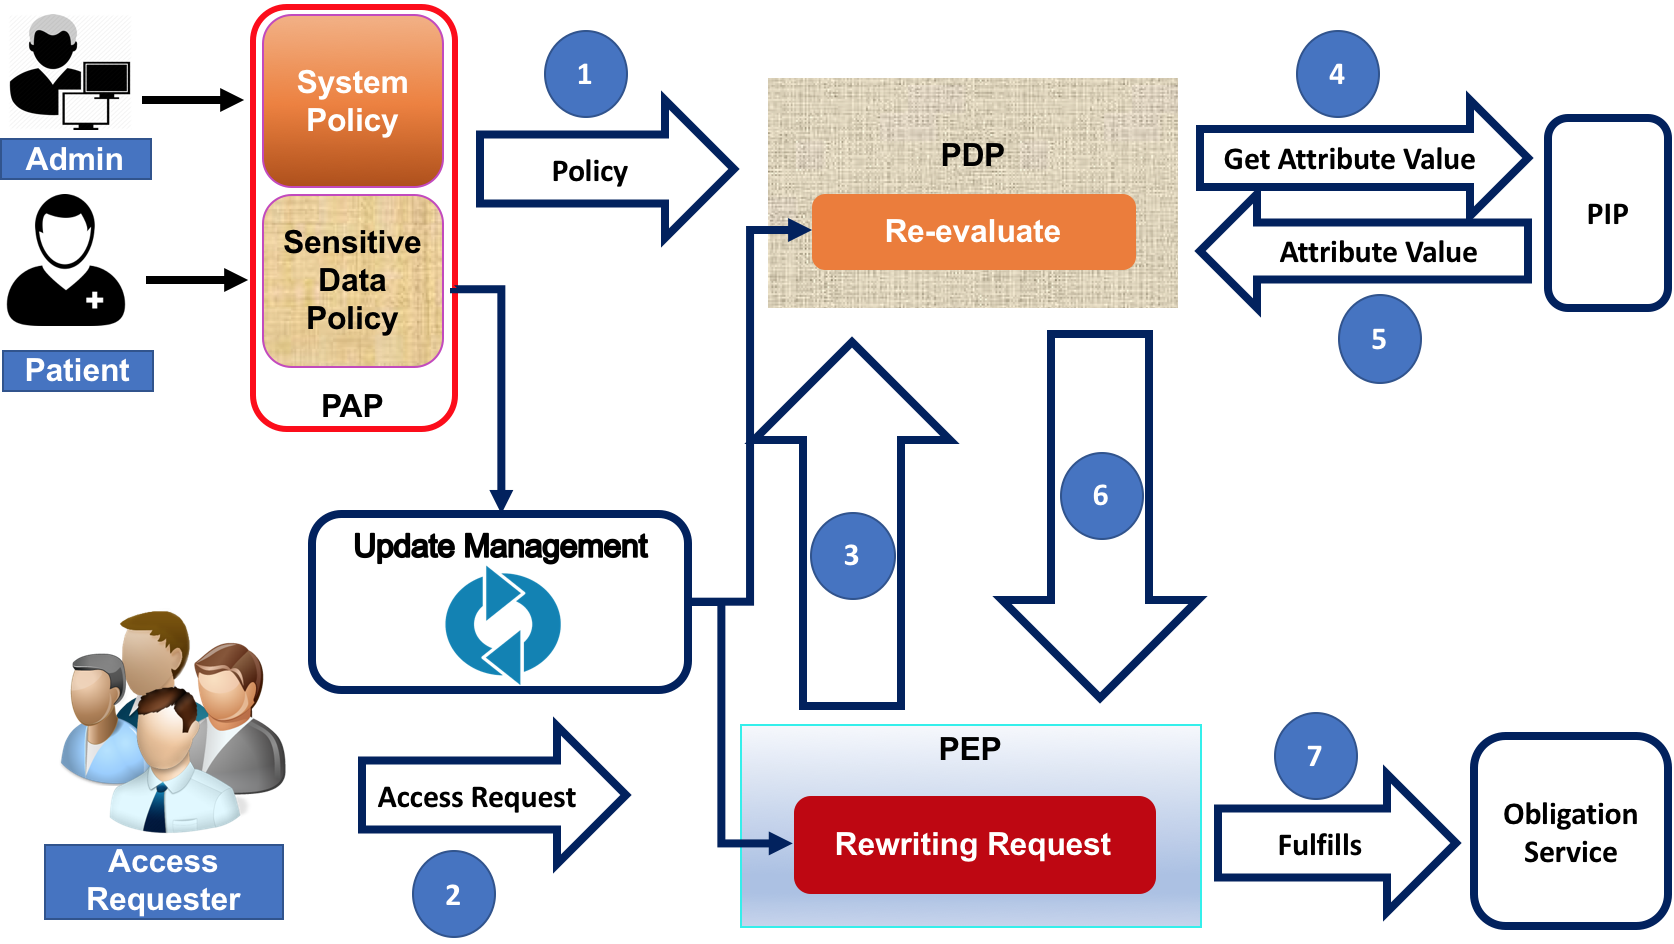
\includegraphics[scale=0.3]{fig/Mainmodel.png}
  \caption{ACDP-HC Model}
  \label{fig.condition}
\end{figure}

The ACDP-HC Model consists of six components:

\textbf{Policy Administrator Points (PAP): }The system entity stores all policies (system policy and sensitive data policies). 
Additionally, PAP converts the entire policy to be stored as \textit{at} and \textit{ac}. 
PAP's work is to provide new policies for PDP and policy updates for UM.

\textbf{Policy Decision Points (PDP): }The system entity evaluates the process, which is the most significant one of the system, where finds the most suitable policy and assigns permissions to access request. 
In addition, PDP containing a sub-entity named re-evaluate request. 
Its duty is to rewrite access request when UM calls for.

\textbf{Policy Information Points (PIPs): }The system entities stores attribute values. 
PIP provides the required attribute values during the evaluation process.

\textbf{Policy Enforcement Points (PEPs): }The system entity receives user requests and formats the request as the tuple $\langle \texttt{attribute - }$ $\texttt{va\\lue} \rangle$.
Then forward to the PDP in oder to evaluate the process. 
In addition, PEP containing a sub-entity is named rewriting request. 
Its duty is rewriting access request when UM calls for. 
%In the event of being impossible to rewrite the query because of insufficient attributes or evidence, PEP will send an authentication request to OS. 
If to rewrite the query because of insuficient attributes or evidence is impossible, PEP sends an authentication request to OS.
%Here, the OS will send these requests to force the users to provide missing attributes and evidence before rewriting the access request.
The OS send these requests to demand the users provide missing attributes and evidence before rewriting the access request.

\textbf{Update Management (UM): }The system entity always listens to changes in the PAP. 
These updates are categorized by UM and then send rewriting or re-evaluating requirements to PEP or PDP.

\textbf{Obligation Service (OS): }The system entity sends a request to the access requester is demanded to fulfill all such requests for a certain period of time before sending the entire return to PEP.

Figure 1 describes the ACDP-HC model in 7 prominent steps:
\begin{enumerate}
  \item The admin or patient sends their policies to the system. These policies are converted into concatenation via the logical operations between $ac$ and $at$.
  \item Internal or External User sends a request to access the system. 
  \item PEP sends all requests after being reformatted for the PDP. Here, PDP evaluate the process.
  \item PDP sends a request for attribute value for PIP.
  \item PIP responds to the value attributes that PDP looks for.
  \item PDP returns the outcome to PEP after the evaluation process ends.
  \item After receiving the response from PDP, PEP will fulfill Obligation Services (if any) before executing the users request.
\end{enumerate}

During the seven steps, ACDP-HC model shows the steps for monitoring the policy update process on the PAP. 
If any changes occur to the available policies in the system, UM proceeds to classify those changes and determine next step by re-evaluating or rewriting the request. 

\subsection{Algorithm}\label{Al}
%This section will introduce the applied key algorithm to our approach. 

\begin{algorithm}
  \caption{Optimized Dynamic Policy Evaluation}
  \label{alg:optimized}
  \fontsize{9pt}{12pt}\selectfont
  \begin{algorithmic}[1]
    \item \textbf{Require:} \textbf{$PAP$:} pap instance; \textbf{$Q$:} request instance\\
    $\langle decision, non\_applied\_policies, applied\_policy \rangle$ = evaluate($Q$, $PAP$)
    \State changes = getPolicyChanges($PAP$, $applied\_policy$)
    \Switch{$changes.type$}
      \Case{$Delete Policy$}
        \State \Return evaluate($Q, PAP, exclude: non\_applied\_policies$)
      \EndCase
      \Case{$Insert Polilcy$}
        \State \Return $decision$
        %\State \Return evaluate($Q, PAP, exclude: non\_applied\_policies$)
      \EndCase
      \Case{$Edit Polilcy$}
        \If{$editConstraints$}
        \State \Return evaluate($Q, PAP, only: applied\_policy^*$)
        \ElsIf{$deleteConstraints$}
        \State \Return evaluate($Q, PAP, only: applied\_policy^*$)
        \ElsIf{$insertConstraints$}
        \State $tempAtt$ = getLackAtt($Q$, $applied\_policy^*$)
        \State  $v$ = Obligation($tempAtt$)
        \State  $Q^*$ = rewiteRequest($Q$,$v$)
        \State \Return evaluate($Q^*, PAP, only: applied\_policy^*$)
        \EndIf
      \EndCase
    \EndSwitch
  \end{algorithmic}
\end{algorithm}

The Algorithm 1 classifies a policy change from their property (\textit{Delete, Insert} or \textit{Edit policy}). 
The \textbf{Require} of this method includes the PAP instance and the access request (line 1).
%K?t thúc quá trình ?ánh giá chính sách, k?t qu? s? ???c l?u tr? vào tuple $\langle decision, non\_applied\_policies, applied\_policy \rangle$ v?i $decision$ tr? v? giá tr? là Permit ho?c Deny, $non\_applied\_policies$ ch?a các policy ?ã xét và applied\_policy là policy gán cho access request.
After the policy evaluation process, the result is stored as the tuple $\langle decision, non\_applied\_policies, applied\_policy \rangle$ where $decision$ returns either \texttt{Permit} or \texttt{Deny}, $non\_applied\_policies$ contains the evaluated policy and applied\_policy is the policy assigned to the access request (line 2).
In line 3, $changes$ is a parameter storing type of change. 
%If the temp's value is "\textit{Delete}", the method find a new policy with the goal of replacing the original policy is deleted.
If the temp's value is "\textit{Delete}", the method which finds a new policy with the goal of replacing the original policy is deleted.
In this process, the $non\_applied\_policies$ policies are ignored (line 5 and line 6). 
In the type of "\textit{Insert}" the new policies are stored in the PAP and the system ignores \textit{Insert} type (line 7,8).
The case of "\textit{Edit}" is divided into three smaller instances: insert rule, delete rule, and edit rule. 
Both delete and edit rule are re-evaluated by the access request with edited policy "$applied\_policy^*$" (from line 10 to line 13).
For the insert rule, the attributes or evidence are found if it does not exist in the request.
If not exist, PEP will send an authentication request to OS. Otherwise, \textit{tempAtt} returns null (line 16). 
Consequently, the Obligation sends these requests to force the users to provide missing attributes and evidence before rewriting and evaluating the access request (line 17 and 18). 
See \cite{son2017rew} for more detail.

\section{Evaluation}\label{sec:eva}

%In this section, we present our research evaluation consisting of two parts. 
%The first part is comparing our proposed model with previous research models. 
%The second part is analyzing the performance of the system when being measured on different scenarios.

\subsection{Comparison: }

In this section, based on several criterias, we compared the ACDP-HC model with the STEM-RBAC model \cite{georgakakis2011spatio}, the extension of the conventional RBAC access control policy - team based access control (TMAC) \cite{georgiadis2001flexible} %which is considered to be the extension of the conventional RBAC access control policy 
and, implementations of the Attribute-Based Access Control (ABAC) - XACML v3.0 \cite{rissanen2013extensible}, %which implements the Attribute-Based Access Control (ABAC). 
The characteristics of these models are shown in Table 1.

\begin{table*}[]
\centering
\caption{Characteristics comparison}
\label{comparision}
\begin{tabular}{|l|l|l|l|l|}
\hline
                                      & \multicolumn{1}{c|}{\textbf{STEM-RBAC}} & \multicolumn{1}{c|}{\textbf{TMAC}} & \multicolumn{1}{c|}{\textbf{XACML v3.0}} & \multicolumn{1}{c|}{\textbf{ACDP-HC}} \\ \hline
\textbf{Fine-Grained Controls} & Medium                                  & Medium                             & High                                     & High                                \\ \hline
\textbf{Robustness}                   & Low                                     & Low                                & High                                     & High                                \\ \hline
\textbf{Dynamic Policy}               & Static                                  & Static                             & Static                                   & Dynamic                             \\ \hline
\textbf{Practicality}                 & High                                    & High                               & Low                                      & High                                \\ \hline
\textbf{Context Information}          & Medium                                  & Low                                & High                                     & High                                \\ \hline
\end{tabular}
\end{table*}

\textbf{Fine-Grained Controls: }
It represents a special characteristic with flexible access control, which supports defining user permissions for the system after successful authentication.  
It is desirable to realize the ease of management without additional or complex manipulation of the access permissions. 
Both ACDP-HC models and XACML v3.0 can support high fine-grained access mechanisms because both models allow the definition of policies to the level of Attribute.

\textbf{Robustness: }
It depends on parameters like flexibility.%, less-error-prone user interface, transparent system etc. 
%In the healthcare system, the most important parameter is flexibility. 
In the proposed approach, this requirement is maximally supported by dynamic policy mechanism. 
In the other models, XACML v3.0 is more flexible because, in addition to supporting spatial and temporal attributes, it supports other attributes.

\textbf{Dynamic Policy: }
This feature is shown by whether the owner policy is allowed to change the policy in real time or not. 
According to Dunlop et al. \cite{dunlop2001dynamic}, a system is supposed to support the dynamic policy only if the following criteria are fulfilled:
\begin{itemize}
  \item Policy includes a variable which contains a reference to run-time or location.
  \item Policy is able to be altered during request time.
  \item Ability to create, update or delete policy during the request time.
  \item Ability to dismiss the policy during the request time.
\end{itemize}
%Considering the criteria above only our model supports dynamic policy.
Considering these criteria, only the ACDP-HC model supports dynamic policy.

\textbf{Practicality: }
It denotes how easy to enforce an access control system in a real-time system.  
The STEM-RBAC, TMAC models and ACDP-HC model are designed specifically for the healthcare system. 
%In another model, currently, there are many implementations of XACML v3.0. 
%XACML v3.0 is implemented in other models.
Currently, there are many implementations of XACML v3.0. 
However, in order to integrate this model into the healthcare system, further research is necessary. 
Hence, practicality of XACML v3.0 is lower than the others.

\textbf{Context Information: }
This characteristic shows how much the access control model can handle the user context. 
%It means that whether permission rights are affected with changes in contexts.
In other words, this characteristic defines whether permission rights are affected by changes in contexts. 
The TMAC model supports merely team components. 
%no other contexts such as object conditions etc. 
Other contexts such as object condition is excluded.
On the other hand, ACDP-HC model supports situation components, including composed of user context and object context. 
%For example, when the user's context occurs changes, the user's attributes can be updated dynamically.
For example, when changes occur in the user's context , the user's attributes can be updated dynamically.

\subsection{Experiments}\label{Evaluate:Exp}

This section describes the experiments are conducted to simulate the policy changes in the healthcare context and profile the process of evaluating requests in the context.
The XACML policies, requests input and the developed simulation will be illustrated before the running profiling is analyzed and discussed.

\begin{figure}[ht!]
  \centering
  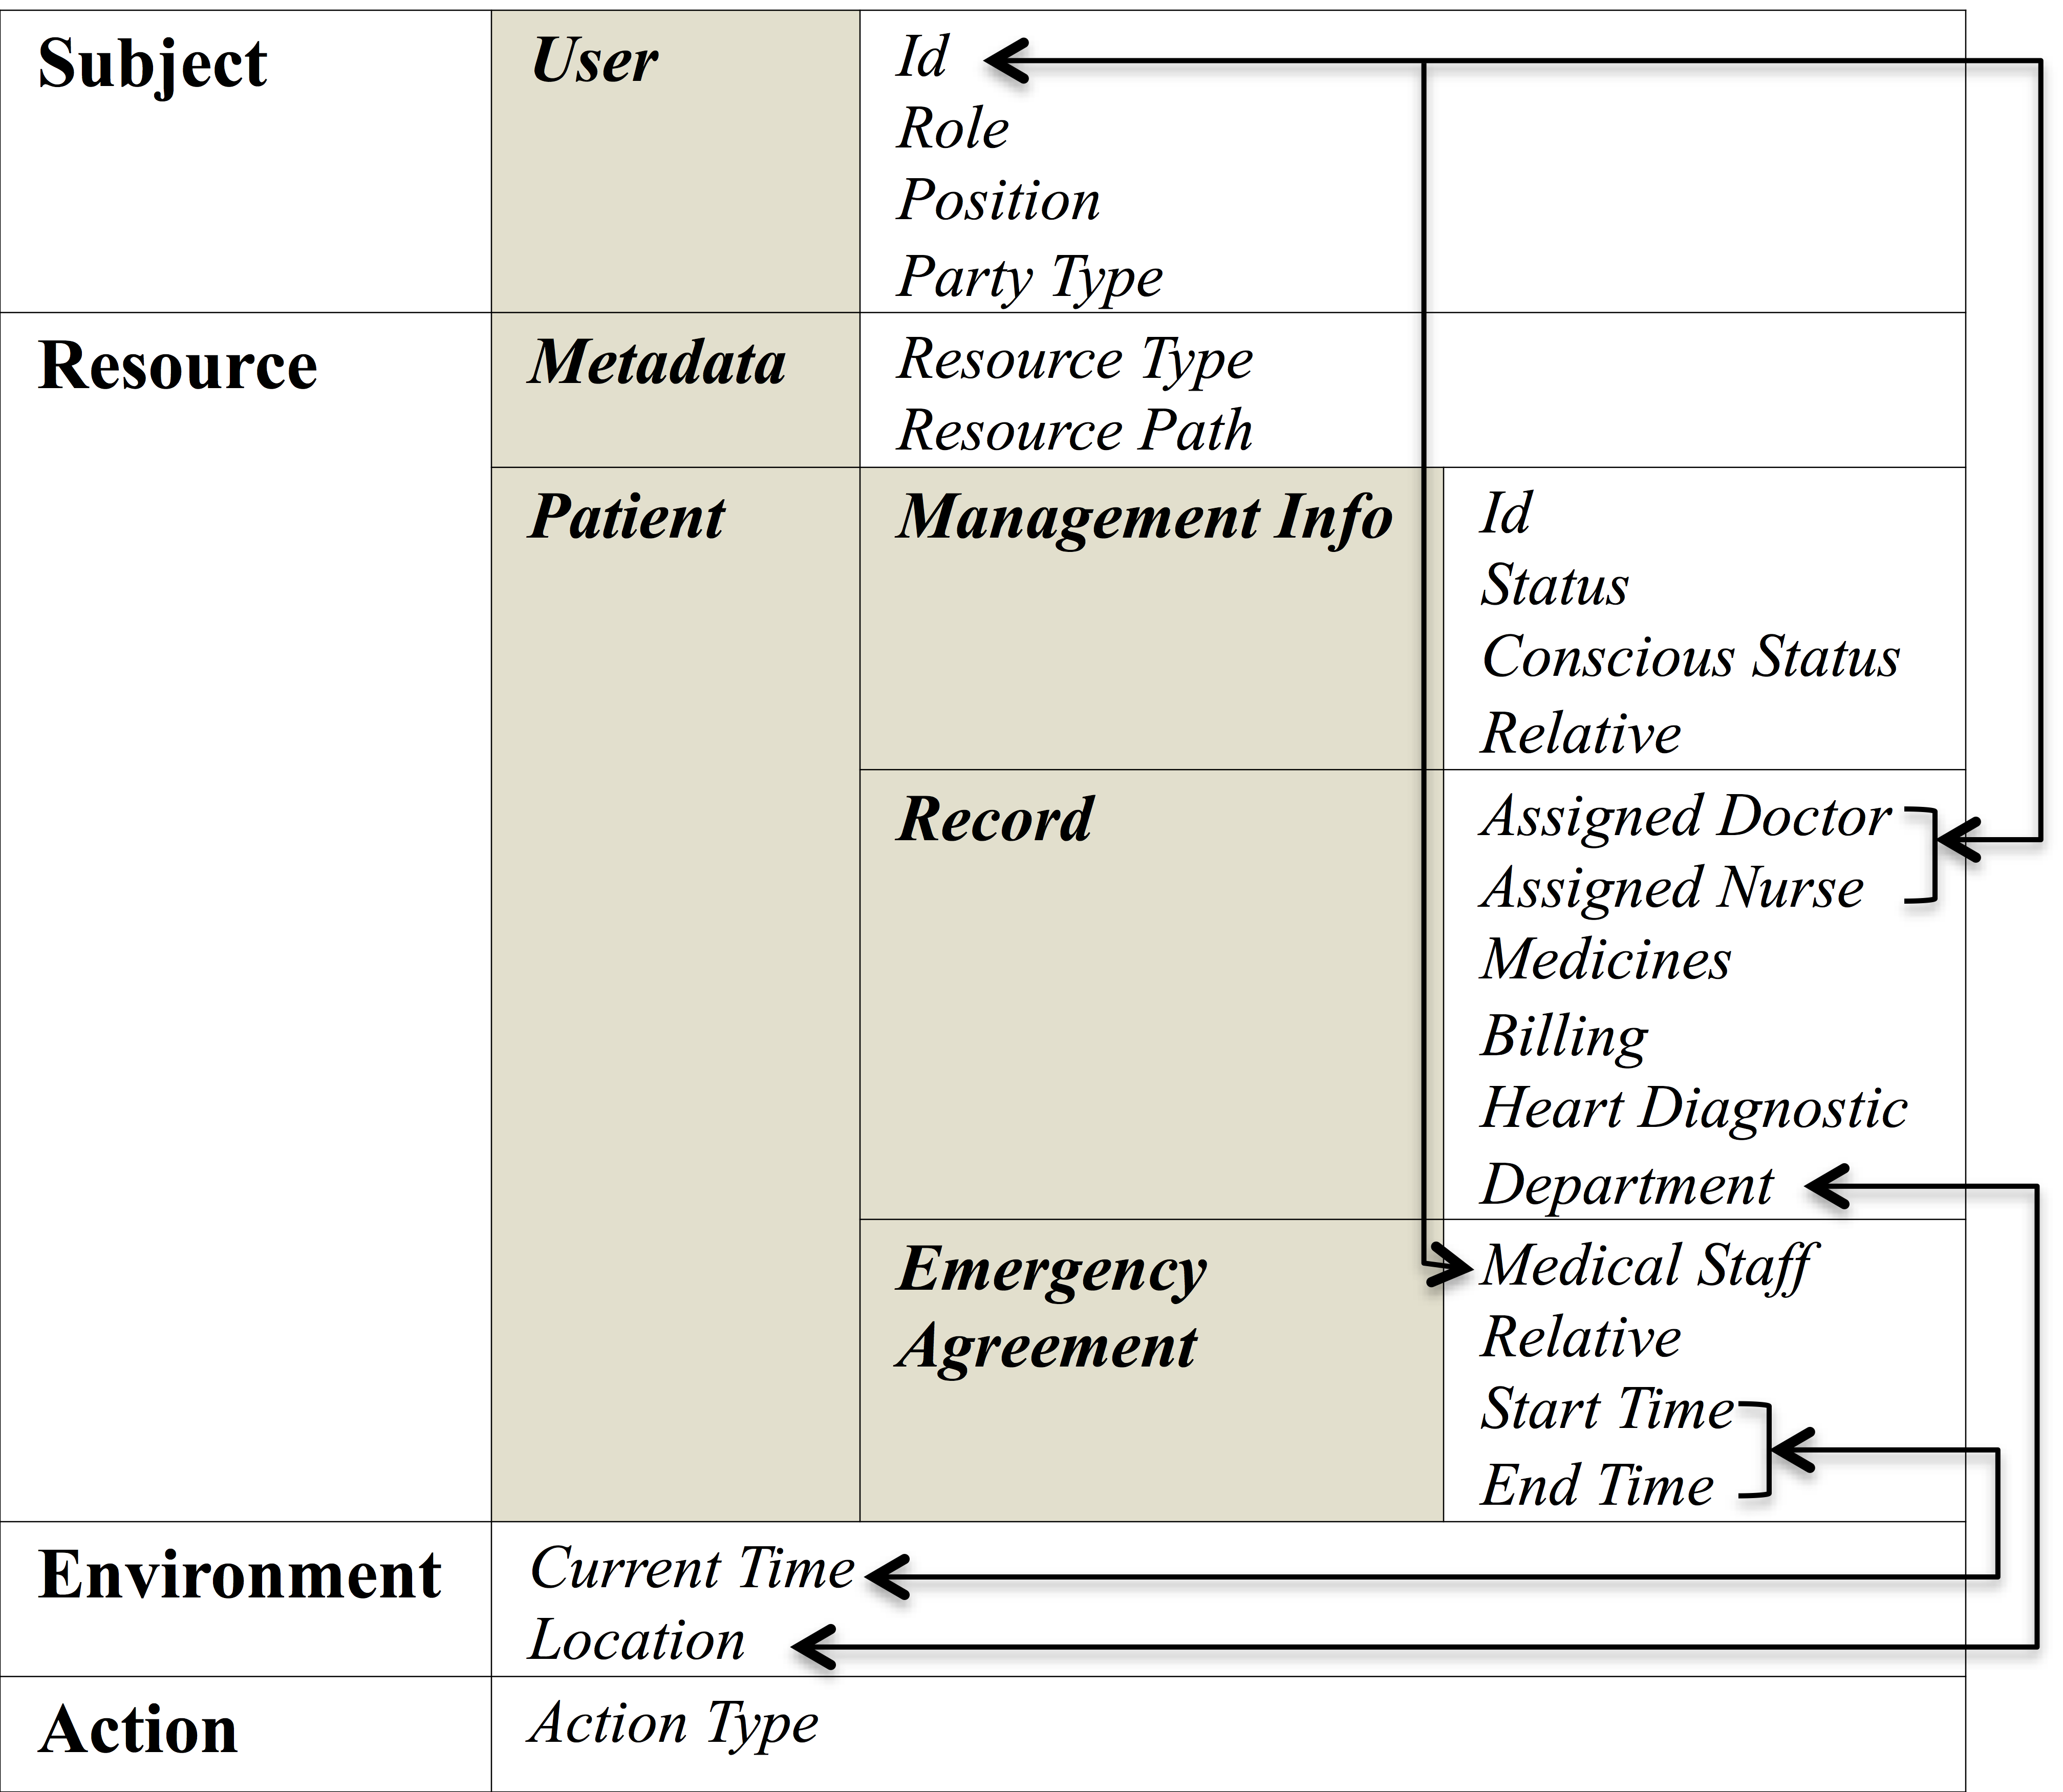
\includegraphics[scale=0.4]{fig/attributes.png}
  \caption{Healthcare Attributes}
  \label{fig:attributes}
\end{figure}

The policies and requests are constructed from attributes in three categories Subject, Resource, Environment and Action which are presented in Figure \ref{fig:attributes}.
The object-oriented approach is used to construct Subject and Resource attributes.
Those are \textit{User.Id, User.Role} and others for Subject. 
For Resource, those are \textit{Patient.Record.Assign-edDoctor, Patient.ManagementInfo.Id} and other such attributes.
From the approach in \cite{medvet2015evolutionary}, policies are constructed based on two kinds of constraint.
One kind of constraint is between an attribute and a value.
Another kind of constraint, relationship constraint is between two attributes in different categories.
Connection lines in Figure \ref{fig:attributes} are instances of this kind of constraint.
The Axiomatic Abbreviated Language for Authorization (ALFA)\footnote{https://www.axiomatics.com/blog/tag/alfa/} is used to specify policies to reduce the verbosity of XML format then guarantee the correctness of the generated policies in the XACML 3.0 standard.
Figure \ref{fig:policyset} illustrates the policy set having the User Emergency Policy created by a patient is in higher priority in request evaluation than the Emergency Policy created by the System Administrator.
Figure \ref{fig:policychanges} illustrates changes to the User Emergency Policy in five cases: the policy Deleted by the Admin, another policy Inserted by the patient and the policy Edited (Delete constraints, Edit constraints and Insert constraints) by the patient.
The policies and requests are loaded and run successfully in both open source XACML implementations Balana and OpenAZ\footnote{https://github.com/khiem111189/balana\\https://github.com/khiem111189/incubator-openaz}.

\begin{figure}[ht!]
  \centering
  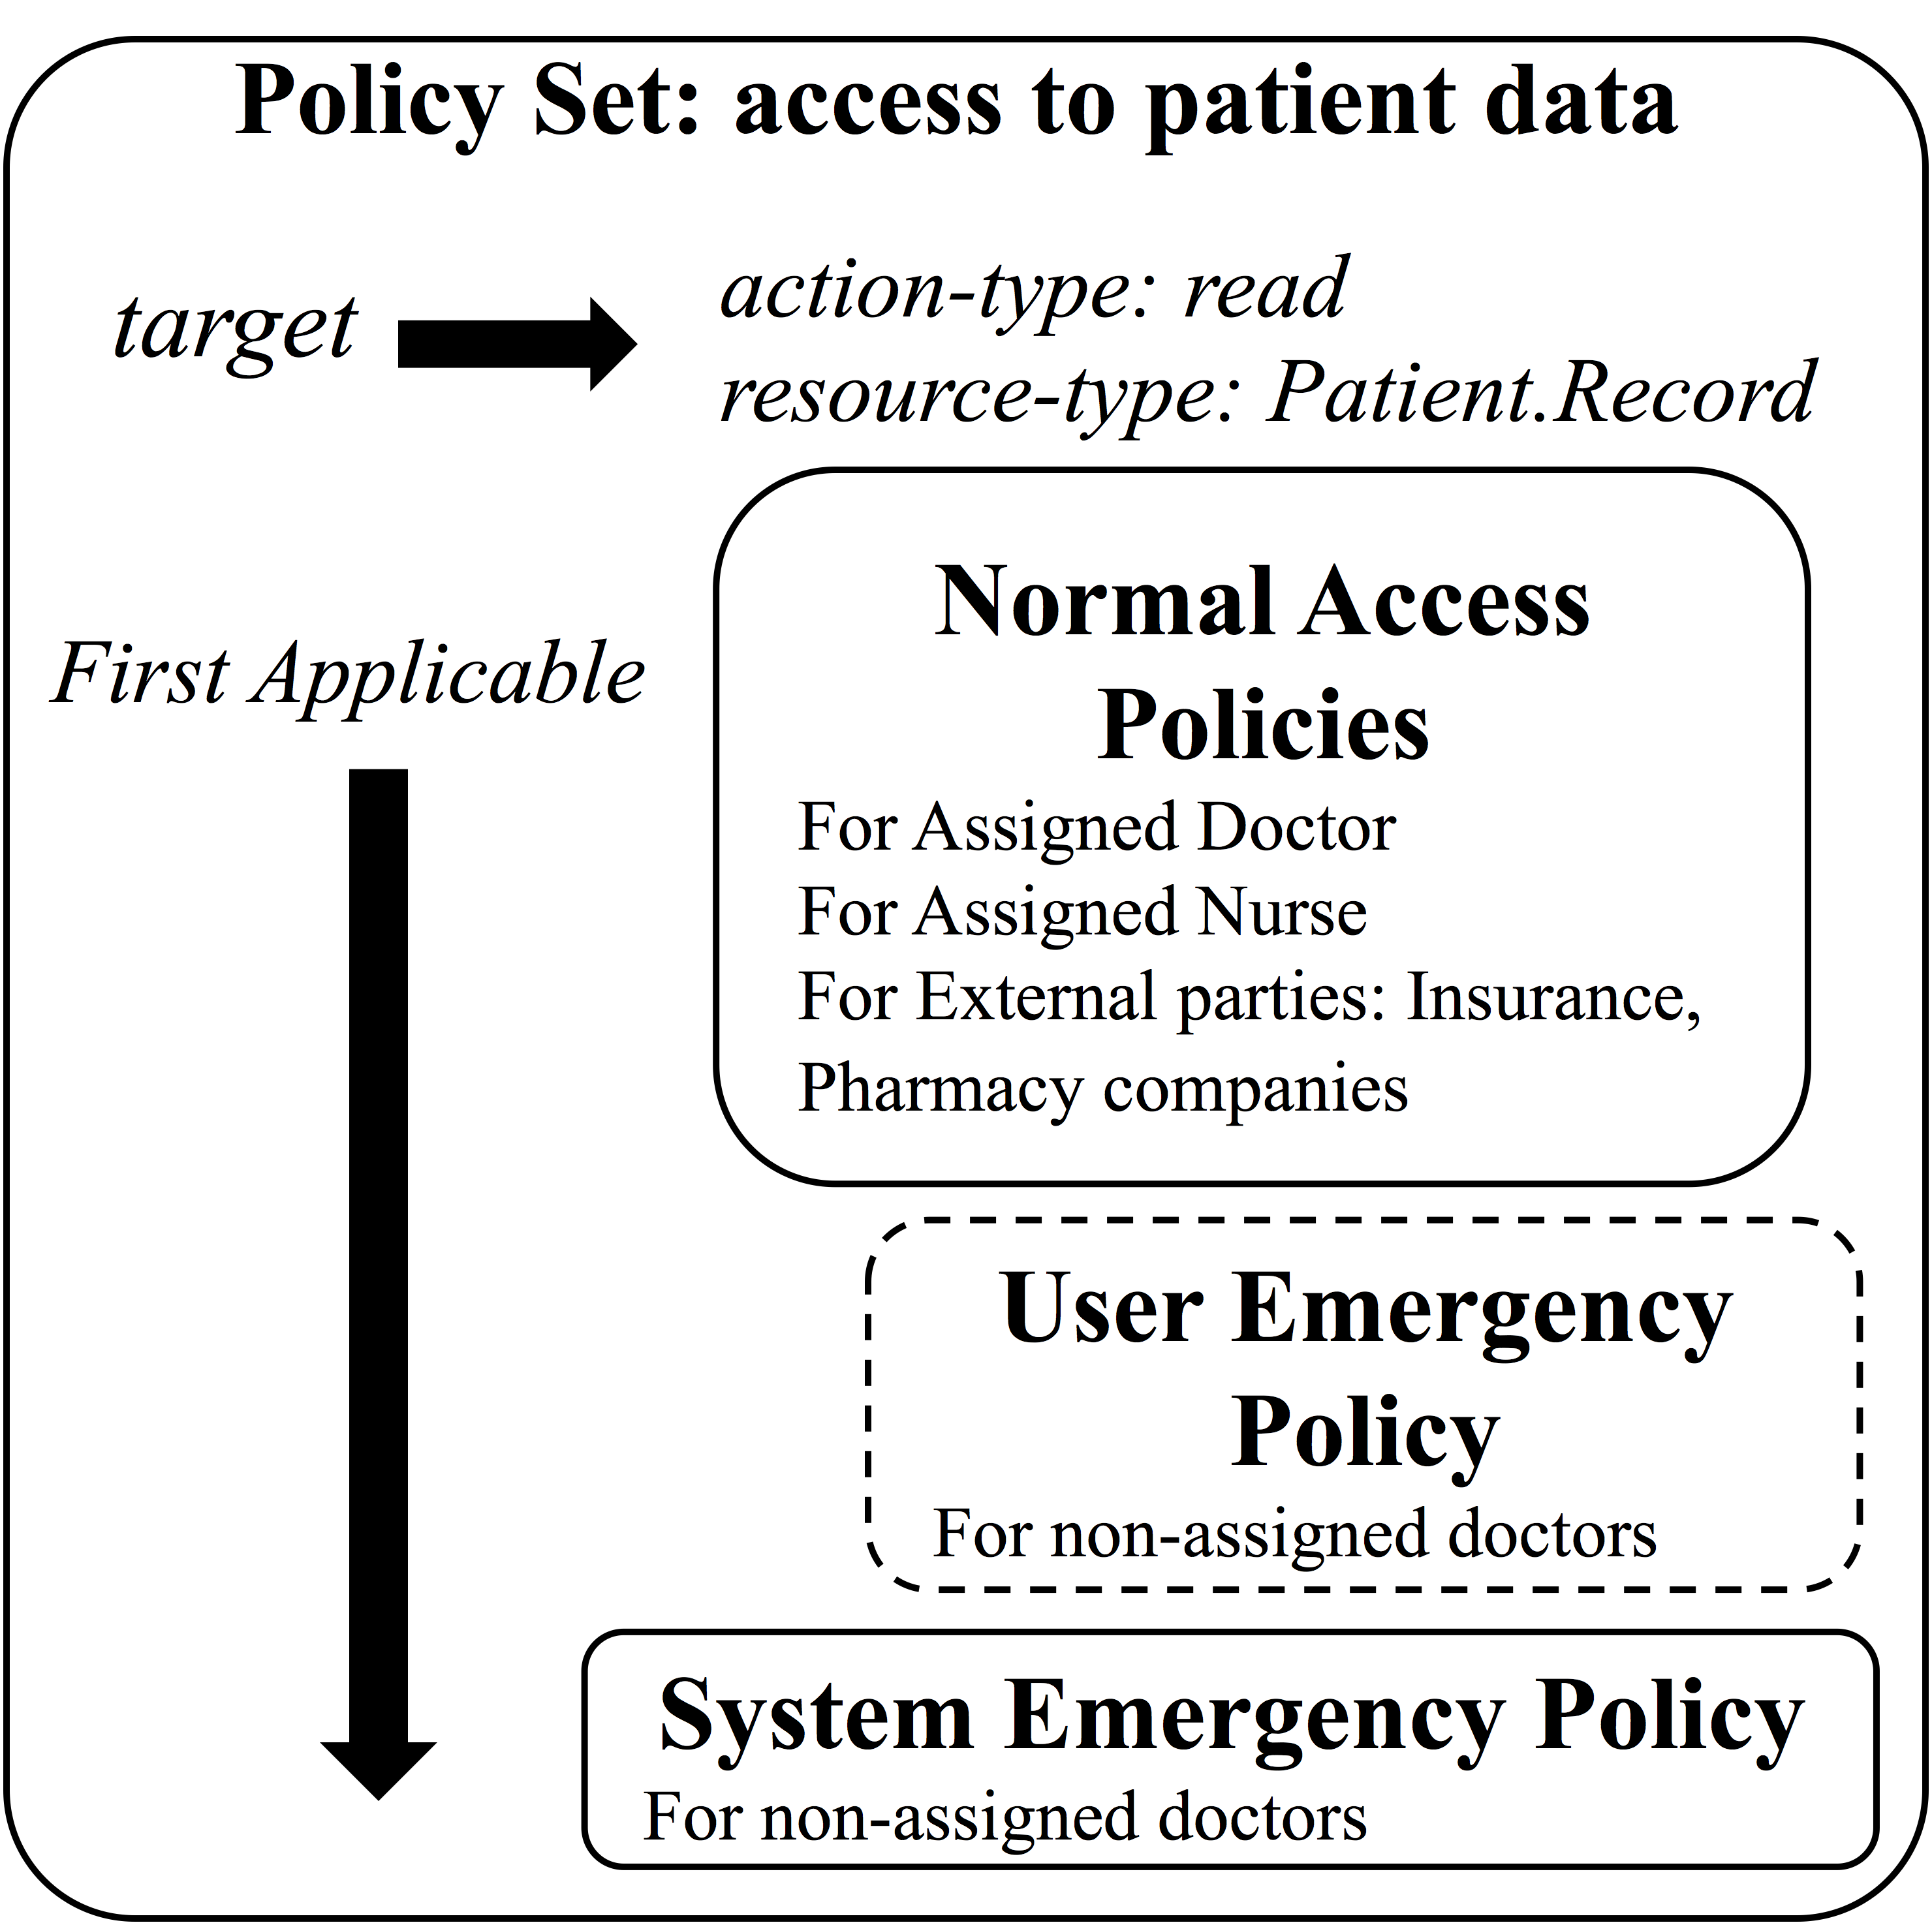
\includegraphics[scale=0.5]{fig/PolicySet.png}
  \caption{PolicySet for Patient Data}
  \label{fig:policyset}
\end{figure}
\begin{figure}[ht!]
  \centering
  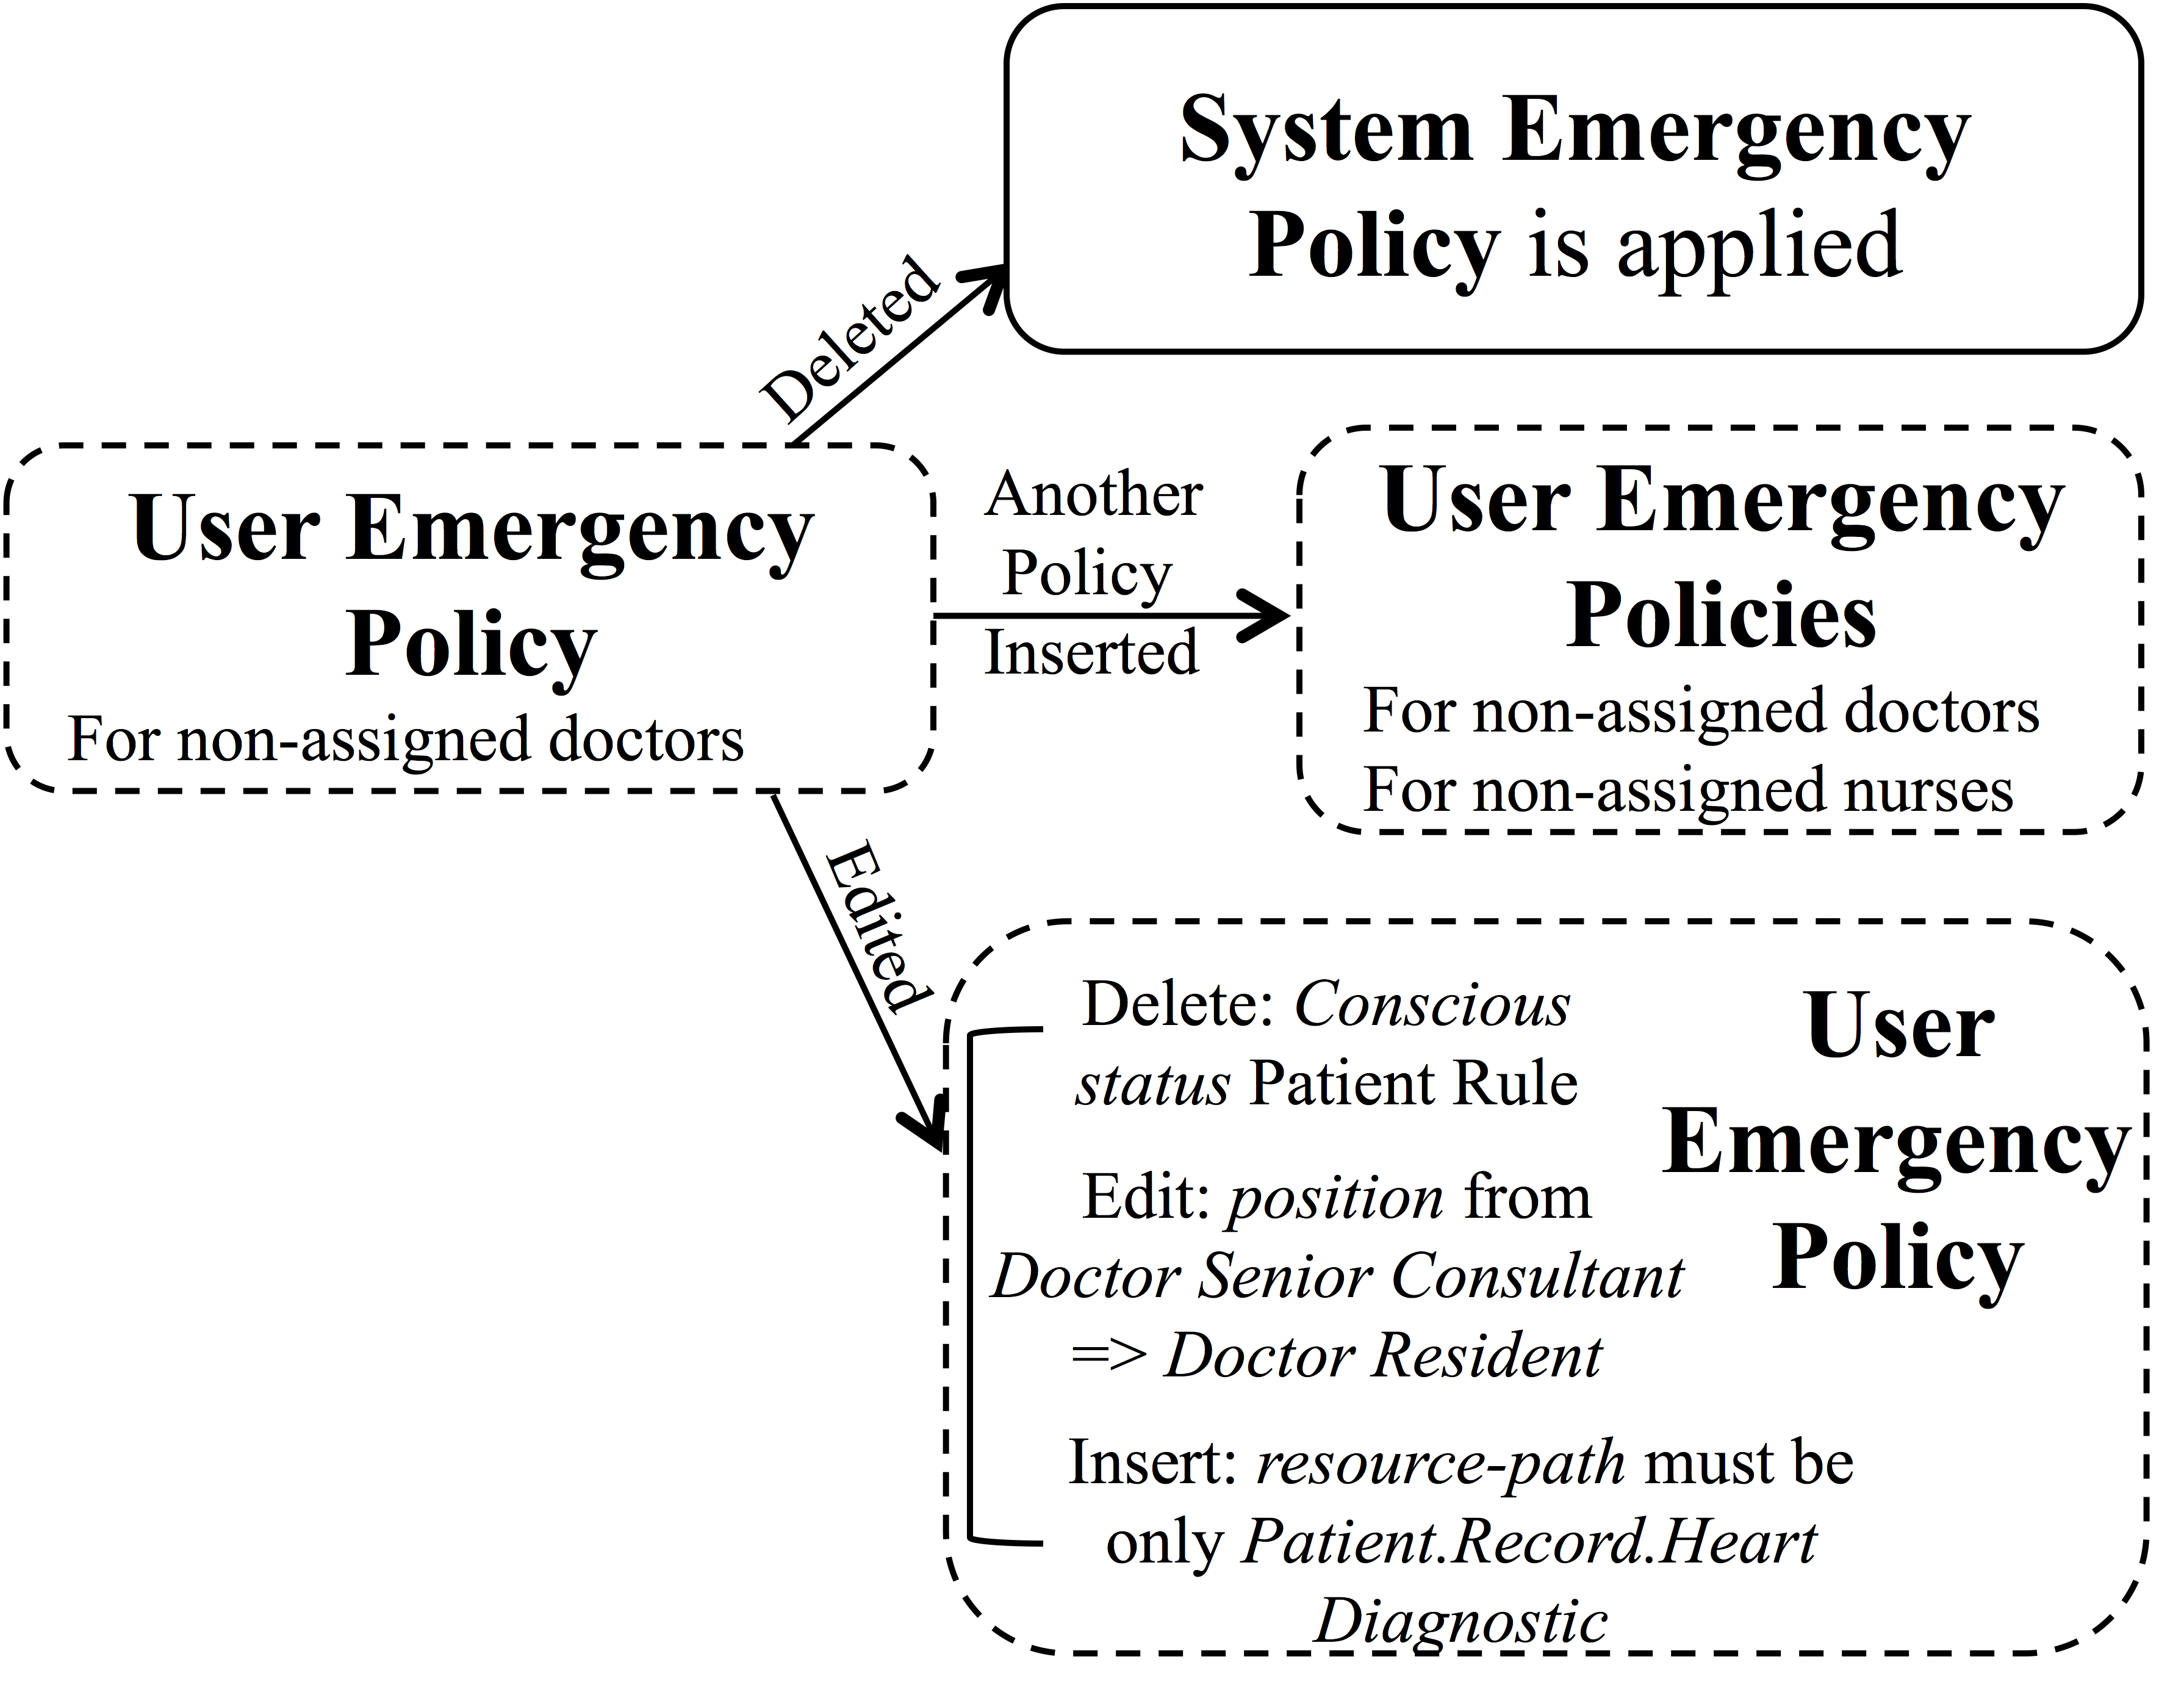
\includegraphics[scale=0.5]{fig/PolicyChange.png}
  \caption{Changes to the User Emergency Policy}
  \label{fig:policychanges}
\end{figure}

The dynamic policy environment is simulated in Java\footnote{https://github.com/khiem111189/research\_group} wrapping the Balana XACML framework as the static policy evaluation engine.
In the dynamic policy environment, before returning the response, it is required to check if there is any policy change event.
If there is no change, the response is proceeded to the client.
If there are changes, there are two approaches to apply.
The \textbf{simple approach} is re-evaluate the request with new policy changes.
The \textbf{optimized approach} is illustrated in Algorithm \ref{alg:optimized}.
There could be a loop of checking policy change event and re-evaluate the request.
Five cases in Figure \ref{fig:policychanges} are used for experimenting those two approaches.
In these experiments the policy change event happens only once.

\begin{figure}[ht!]
  \centering
  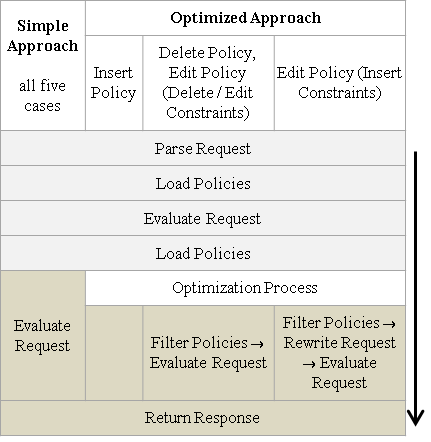
\includegraphics[scale=0.8]{fig/actions.png}
  \caption{Healthcare Attributes}
  \label{fig:actions}
\end{figure}

The running experiments are profiled into process actions illustrated in Figure \ref{fig:actions}.
The \textbf{optimized approach} introducing the \textit{Optimization Process} action brings advantages on relinquishing the re-evaluation for the Insert Policy case; reducing the complexity of policies for the re-evaluation in the Delete Policy and Edit Policy case or improving the throughput by re-writing the original request with addition attribute values.
However, the action \textit{Filter Policy} does not reduce the total expending time of \textit{Evaluate Request} actions less than the total one for the \textbf{simple approach}.
The reason is that Balana evaluates request mostly one millisecond with different experimented policy sets.
The system configuration for the experiments is a 64-bit machine with 8GB of RAM and 2.8 GHz Intel Core i5 CPU running macOS High Sierra.
Moreover, actions inside the \textit{Optimization Process} may cause new potential security problems to the whole evaluation process in comparison to only re-evaluating the original request of the \textbf{simple approach}.

\section{Related Work}\label{sec:prior}
%This section briefly outlines the prior work of balancing between the rigorous nature of access control systems and the prioritization of care delivery in the medical environment.

In traditional access control models such as Discretionary Access Control (DAC), Mandatory Access Control (MAC) or Role-Based Access Control (RBAC), the user privileges must be defined in advance and set a limited number of changes throughout the system implementation.
Therefore, a great number of studies have extended the RBAC model in order to meet specific requirements in the medical setting. 
Garcia-Morchon and Wehrle  have suggested a Context-Aware Role-Based Access Control (CA-RBAC) model \cite{garcia2010modular} in order to raise awareness of context and to adapt its security properties in order to ensure the users' safety. 
%One of the disadvantages of this model is that there is no preventive or detection mechanisms as well as a verification process to check whether a user's access is correct or wrong when an emergency arises. 
The disadvantages of CA-RBAC model is the lack of preventive or detection mechanisms as well as a verification process to check the correctness of user's access in emergency context.
Similarly, Georgakakis et al. introduced Spatio temporal emergency role based access control model (STEM-RBAC) \cite{georgakakis2011spatio}. 
The emergency access mechanism was recommended by the author.
Additionally, STEM-RBAC model allows exception-albeit controlled access in the event of an emergency, using role hierarchies.
A modular security monitor is switched on to monitor abnormal access (in case of an emergency). 
Kabbani et al. \cite{kabbani2014specification}  introduced a Dynamic Authorization model based on the XACML v3.0 model. 
%which adds to the flexibility situations of traditional XACML modeling and can address the changes that occur in the healthcare system. 
The Dynamic Authorization model adds to the flexibility situations of traditional XACML modeling and addresses the changes that occur in the healthcare system.
In this model, the situation changing detection function is always enabled to receive change information from the external environment and to select the appropriate situation. 
The weakness of Dynamic Authorization model, however, is that all situations must be defined in advance and it does not support dynamic policy.
%Following our approach, the model extended is called Attribute-based Access Control.
%With this model, the policies are hereby defined highly detailed and easy to express complex scenario in the real system. 
%Moreover, with the support permitting the admin and the patients to update the policies also make our approach more flexible.

Yu et al. \cite{yu2011fdac} proposed a Fine-Grained Distributed Data Access Control (FDAC) model based on Attribute-Based Encryption. 
%The key idea is providing a distributed data access control possibly assisting in monitoring effectively on the sensor data. 
A network controller, containing access structures, acts as a central distribution center and distributes keys to the users in FDAC. 
%This approach may reduce the likelihood that BTG will lead to emergencies or exceptions. 
This approach may reduce the possibility that BTG leads to emergencies or exceptions.
However, FDAC model is based on a centralized approach because only the network controller can perform the key management. 
%If the network controller is compromised, there will be no security provision in the network, which is a single point of failure. 
If the network controller is compromised, provision in the network is not secured, which is a single point of failure.
To avoid a single point of failure, Ruj et al. \cite{ruj2011distributed} proposed a multi-authority Attribute-Based Encryption (MABE) - a based access control plan. 
Their goal is to provide complete distributed data access control using a number of Distribution Centers (DCs). 
%All access structures from each DC, need to satisfy the attributes from the sensor nodes, are ANDed together to obtain full access to a single user. 
However, this approach does not explain in detail how to combine all access structures. 
Without a combined approach, the users must store all access structures to access different types of data from the sensor network. 
%Maw et al. \cite{maw2013adaptive} has proposed an Adaptive Access Control (A2C) access control model with priority and behavioral monitoring to provide effective access control for medical data in which the users can override denied access, when unexpected events occur. 
Maw et al. \cite{maw2013adaptive} proposed an Adaptive Access Control (A2C) access control model. 
The A2C  model obtains priority and behavioral monitoring to provide effective access control for medical data,
In A2C model ,users can override denied access when unexpected events occur.
%In addition, the trust model of user behavior is used to test the user's actions, location, and time, but there is no detailed model of behavior. 
In addition, the trust model of user behavior is used to test the user's actions, location, and time, except the user's behavior. 
Without a trusting behavior model, access decisions can not be conducted effectively (limited). 
Some access control models for medical data such as FDAC, A2C and MABE use cryptographic methods to store data and control access to data. 
Nevertheless, systems need to predefine access, roles, as well as policies prior to deployment. 
%However, it is difficult to prioritize possible needs for accessing real-world applications. 
Prioritizing possible needs for accessing real-world applications is challenging in these models.
%In fact, there might be unanticipated situations at any time.
Obviously, unanticipated situations might occur spontaneously.
%For real world applications, the system needs to be flexible enough to make decisions on data access based on unusual circumstances beyond normal circumstances. 
For practical applications, the system needs to be flexible enough to make decisions on data access based on unusual circumstances beyond normal circumstances.
%Therefore, in our approach, centrally stored data is taken from various sources (sensor devices, even from a different department, possibly another hospital). 
%Therefore, centralized data encryption is not appropriate for our approach; instead, we exploit security by allowing patients to create secure policies for all data considered as sensitive one. 
%Another reason for us ignoring data encryption is that cryptography-based access control is designed for unreliable environments where the lack of global knowledge and control are defining characteristics \cite{maw2014evaluation}. 

Ardagna et al. \cite{ardagna2008regulating} introduced a new approach addressing the problem of balancing strict nature of traditional access control systems. 
The author defines the policy space regulating access to medical data and describes how policies are identified and enforced in each space and their combinations. 
The author approach governs all access; otherwise, they will fall into a "BTG policy", and aim to better handle "abnormal" access requests \cite{ardagna2010access}. 
In this paper, the description defines the data space of a policy into four different spatial regions: Access (P+), Access is denied (P-), Planned Exceptions (EP), and Unplanned Exceptions (EU). 
%One of the drawbacks is that the author's approach only supports the combining algorithm as "First-Applicable" for policies. 
Regretfully, this approach only supports the combining algorithm as "First-Applicable" for policies. 
%This greatly influences the design of scenarios between policies because it is impossible to anticipate all the activities (normal and urgent situations) that may occur in the healthcare system. 
This limitation influences the design of scenarios between policies because to anticipate all the activities (normal and urgent situations) that may occur in the healthcare system is impossible. 
Another disadvantage is that unauthorized users can access an emergency situation in some sensitive instances \cite{balasubramaniam2013white}. 
This model needs some secondary policies for each case to meet the privacy requirements.

%Liu et al. \cite {liu2017btg} introduces the BTG-Biba model that improves and extends from the original Biba model, primarily by solving the cross-domain problem. 
%The proposed model also brings context and fine-grained control to the system. 
%In addition, this approach enhances the ability to handle system emergency situations. 
%However, this model does not support the selective sharing function of the EPHR, so it can not support better access control. 
%For this reason, these team proposed a new paradigm that combines the traditional RBAC model with the transformation \cite{liu2016ts}. 
%One of the most prominent weaknesses in these models is that they do not support Dynamic Policy. 
%This feature is strongly supported in our approach, which is the opposite of these previous models.

\section{Conclusion}\label{sec:conclusion}

This paper has proposed risk reduction strategies when emergency situation occurs. 
The approach based on authorized access is granted by the patients through creating sensitive data policies. 
%If there is an unauthorized intrusion of private data, almost all the operations from access requester will be recored and be responsible for them.
%If an unauthorized access to medical data is detected, all the operations from the users will be recorded and be responsible for them.  
If an unauthorized access to medical data is detected, all the operations from the users will be recorded and be analyzed.
The strength of the proposed system is that it allows admins and patients freely to change policies during evaluation process or to grant access to another user. 
%Supporting flexibility to a maximum extent is the goal. 
%Besides, the healthcare system is extraordinarily complicated, where each user can change positions, roles, and attributes on a regular basis. 
The approach of this paper is a policy update application that could meet access requirements in emergency situations, which can not be accessed under normal circumstances. 
In this way, the approach will minimize the BTG in emergency situation.
Besides, the healthcare system is complicated because each user can change positions, roles, and attributes on a regular basis.
Supporting flexibility to a maximum extent is the main goal in our proposed model. 
%Furthermore, when compared the prior models, ACDP-HC model is better and %whereas retaining required security features of medical data. 
Furthermore, in comparition to prior models, ACDP-HC model provides solution for current shortages. 
%the measurements show that this is a promising approach.
The measurements during the implementation indicate that ACDP-HC model is a promising approach for further application.

%As part of our forthcoming work, we are about to implement a mechanism of detecting conflict and redundancy when updating policies or adding new ones.
The forthcoming study will focus on implementing a mechanism of detecting conflict and redundancy when updating policies or adding new ones. 
%Moreover, we will create policy templates that can better support admin and provide additional features that identify changes to the external environment to provide hints for admin and patients to change policy. 
Moreover,  policy templates will be created to support admin better and provide additional features. 
The main aim is to identify changes to the external environment in order to provide hints for admin and patients to change policy. 
%In addition, we will also consider applying the system in a specific hospital in the future.
In addition, applying the system in a specific hospital in the future is considered as well.


\section*{Example References}\label{sec13}

\subsection{Websites}\label{subsec13.1}

\begin{enumerate}
\item[{[1]}] `Author Guide - IET Research Journals',
http://digital-library.theiet.org/journals/author-guide, accessed 27
November 2014\vspace*{6pt}

\item[{[2]}] `Research journal length policy',
http://digital-library.theiet.org/ files/research\_journals\_length\_policy.pdf,
accessed 27 November 2014
\end{enumerate}

\subsection{Patent}\label{subsec13.2}

\begin{enumerate}
\item[{[3]}] `ORCID: Connecting research and researchers', http://orcid.org/,
accessed 3 December 2014\vspace*{6pt}

\item[{[4]}]
`Fundref', http://www.crossref.org/fundref/, accessed 4 December 2014
\end{enumerate}

\subsection{Journal articles}\label{subsec13.3}

\begin{enumerate}
\item[{[5]}] Smith, T., Jones, M.: 'The title of the paper', IET Syst. Biol., 2007,
1, (2), pp. 1--7\vspace*{6pt}

\item[{[6]}] Borwn, L., Thomas, H., James, C.,~et al.:'The title of the paper, IET
Communications, 2012, 6, (5), pp 125-138
\end{enumerate}

\subsection{Conference Paper}\label{subsec13.4}

\begin{enumerate}
\item[{[7]}]
Jones, L., Brown, D.: 'The title of the conference paper'. Proc. Int.
Conf. Systems Biology, Stockholm, Sweden, May 2006, pp. 1--7
\end{enumerate}

\subsection{Book, book chapter and manual}\label{subsec13.5}

\begin{enumerate}
\item[{[8]}] Hodges, A., Smith, N.: 'The title of the book chapter', in Brown, S.
(Ed.): 'Handbook of Systems Biology' (IEE Press, 2004, 1st edn.), pp. 1--7\vspace*{6pt}

\item[{[9]}]
Harrison, E.A., and Abbott, C.: 'The title of the book' (XYZ Press,
2005, 2nd edn. 2006)
\end{enumerate}

\subsection{Report}\label{subsec13.6}

\begin{enumerate}
\item[{[10]}] IET., 'Report Title' (Publisher, 2013), pp. 1-5\vspace*{6pt}

\item[{[11]}] Brown, F.: 'The title of the patent (if available)'. British Patent
123456, July\vadjust{\pagebreak} 2004

\item[{[12]}] Smith, D., Hodges, J.: British Patent Application 98765, 1925
\end{enumerate}

\subsection{Thesis}\label{subsec13.7}

\begin{enumerate}
\item[{[13]}]
Abbott, N.L.: 'The title of the thesis'. PhD thesis, XYZ University,
2005
\end{enumerate}

\subsection{Standard}\label{subsec13.8}

\begin{enumerate}
\item[{[14]}] BS1234: 'The title of the standard', 2006
\end{enumerate}

\begin{table}[!h]
\fwprocesstable{Example of large table\label{tab2}}
{\begin{tabular*}{\textwidth}{@{\extracolsep{\fill}}lccc}\toprule
Column heading 1 &Column heading 2 & Column heading 3  & Column heading 4\\
\midrule
Result 1 &123 &123 & 123 \\
Result 2 &123 &123 &123 \\
Result 3 &123 &123 &123 \\
Result 4 &123 &123 &123 \\
Result 5 &123 &123 &123 \\
Result 6 &123 &123 &123 \\
Result 7 &123 &123 &123 \\
Result 8 &123 &123 &123 \\
\botrule
\end{tabular*}}{}
\end{table}

\vfill\pagebreak

\section{Appendices}\label{sec14}

Additional material, e.g. mathematical derivations, tables and figures
larger than half a page that may interrupt the flow of your paper's argument
should form a separate Appendix section (see Table~\ref{tab2}). Do not, however, use
appendices to lengthen your article unnecessarily as this section is
included in the word count. If the material can be found in another work,
cite this work rather than reproduce~it.
The appendix section should be in double column format, and come after the references.

\end{document}
